\documentclass[11pt]{report}
\newcommand{\titl}{Machine Learning}
\usepackage[pdftex]{graphicx}
% \usepackage[square,closed,nolabel,light]{OTtablx}
\usepackage{henrian-more}
% \usepackage{tikz}
% \usetikzlibrary{trees,positioning,arrows}
% \usepackage{bbding} % \HandRight


% % from Steve Hicks, via http://anthony.liekens.net/index.php/LaTeX/SubscriptAndSuperscriptInTextMode
% \makeatletter
% \newcommand\textsubscript[1]{\@textsubscript{\selectfont#1}}
% \def\@textsubscript#1{{\m@th\ensuremath{_{\mbox{\fontsize\sf@size\z@#1}}}}}
% \newcommand\textbothscript[2]{%
%   \@textbothscript{\selectfont#1}{\selectfont#2}}
% \def\@textbothscript#1#2{%
%   {\m@th\ensuremath{%
%     ^{\mbox{\fontsize\sf@size\z@#1}}%
%     _{\mbox{\fontsize\sf@size\z@#2}}}}}
% \def\@super{^}\def\@sub{_}

% \catcode`^\active\catcode`_\active
% \def\@super@sub#1_#2{\textbothscript{#1}{#2}}
% \def\@sub@super#1^#2{\textbothscript{#2}{#1}}
% \def\@@super#1{\@ifnextchar_{\@super@sub{#1}}{\textsuperscript{#1}}}
% \def\@@sub#1{\@ifnextchar^{\@sub@super{#1}}{\textsubscript{#1}}}
% \def^{\let\@next\relax\ifmmode\@super\else\let\@next\@@super\fi\@next}
% \def_{\let\@next\relax\ifmmode\@sub\else\let\@next\@@sub\fi\@next}
% \makeatother

% \long\def\footnotesymbol[#1]#2{\begingroup%
% \def\thefootnote{\fnsymbol{footnote}}\footnotetext[#1]{#2}\endgroup}

\begin{document}

\section*{Data generation}

There are basically three priors that I used to generate my training data: $\pi$, $\mu$, and $\Sigma$. $\pi$ is a vector with as many items are there are clusters, and I am using only two clusters for most of this report. $\mu$ is two vectors, two to match the number of clusters, and the vectors are each as long as the number of dimensions of the data, which, for most of this report, is also two. $\Sigma$ is two matrices, symmetric and positive definite.

While I could have used a simple draw from the uniform U(0, 1) for $\pi$, I wanted to handle additional clusters easily, so I drew from a standard Dirichlet distribution (parameters of all ones). Matlab has no Dirichlet function that I could find, so I simply used Gammas draws and normalized.

I drew each $\mu$ from the standard normal distribution ($\mathcal{N}(0, 1)$). The $\Sigma$ was also generated by the standard normal, and then multiplied by its transpose to ensure that it was symmetric and positive definite.

The number of samples I drew varied. Below fifty, my results started to become much less predictable. For most of the report, I am using 1000 samples.
I visually evaluated the variety of samples I was getting by using a simple scatter plot, and the degree to which the clusters overlapped or not, on different runs with different draws of priors and data, seemed to be suitable.

\begin{figure}[h]
  \centering
  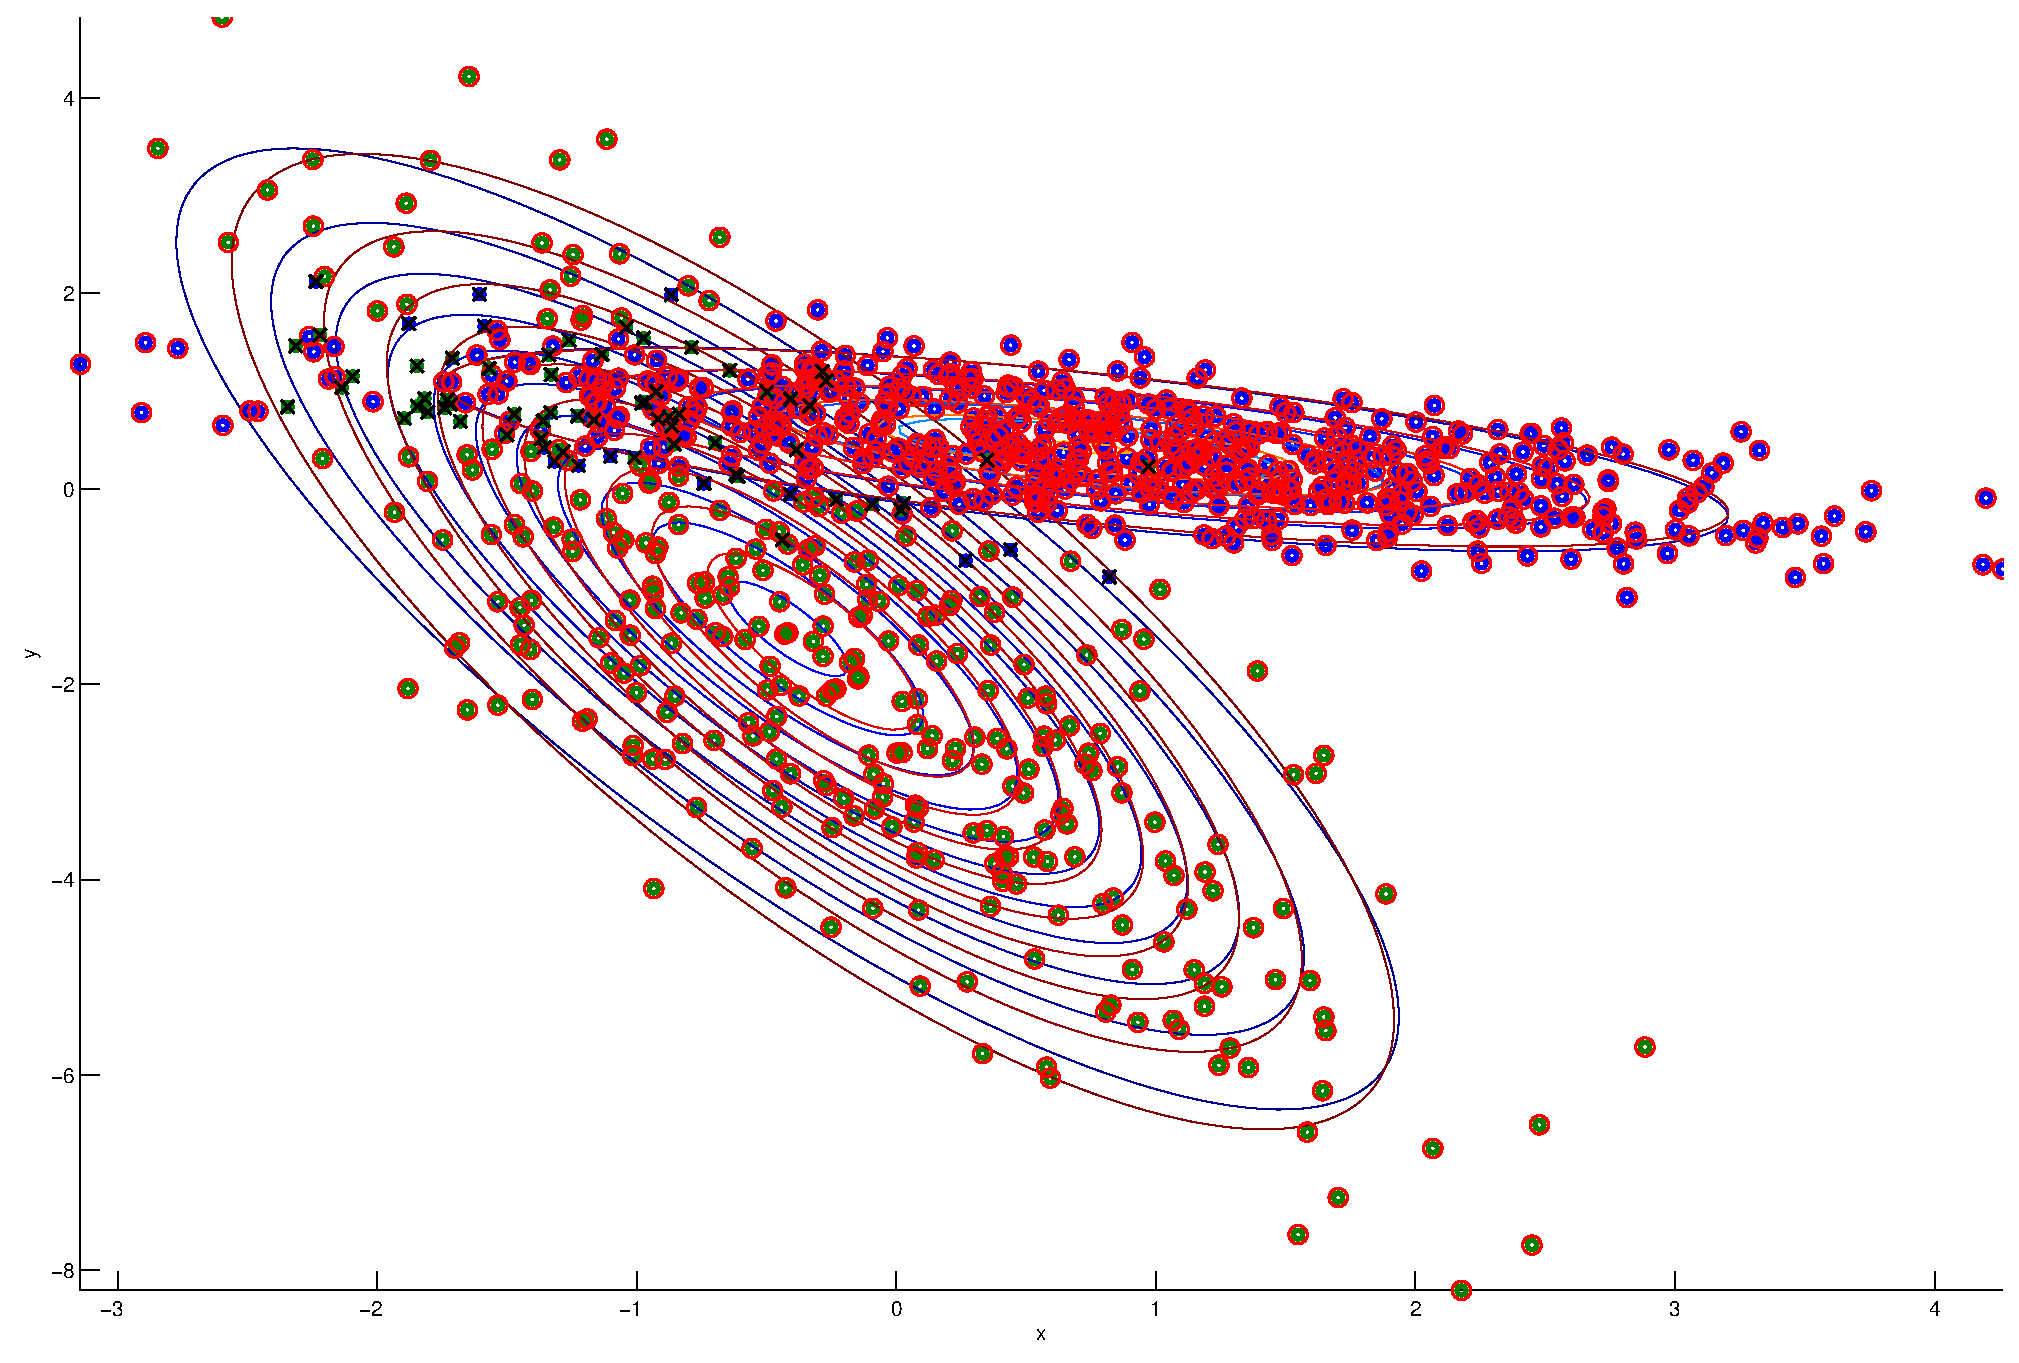
\includegraphics[width=\textwidth]{2x2plot1.eps}
  \caption{Two clusters, two dimensions, 1000 samples. Circles of red indicate correct assignment after last iteration, while a black `x' indicates incorrect assignment. Data from the cluster 1 is colored blue, and points from cluster 2 are colored green. The contours reflect the parameters; blue contours are the parameters used to generate the data, red contours are the result of the EM algorithm.}
  \label{2x2plot1}
\end{figure}

\section*{Expectation Maximization}

I used the Matlab \texttt{kmeans} function to initialize cluster parameters (I evaluated the mean and covariance of each cluster k-means picked out). However, I also found that purely random starts (using the same generation parameters used to generate the data) did not differ much from k-means, except that the log-likelihood would not increase quite so steeply in the first few iterations.

The expectation step was straightforward with \texttt{mvnpdf}. However, my $\Sigma$ parameter would sometimes drop to all zeros, which would throw an error in \texttt{mvnpdf}, in which case I restarted $\Sigma$ for that cluster.

I was able to optimize the estimation of the new $\mu$ parameter for each cluster in the Maximization step, using linear algebra instead of a for-loop, but I couldn't figure out how to optimize the $\Sigma$ estimation step using linear algebra.

I defined my convergence criterion as an increase in log likelihood of less than 0.001, which seems kind of arbitrary, but works well enough (I tried several values). I still had a hard limit of a 100 iterations, for cases of extreme overlap between clusters.

Because of label switching, I chose the assignment of labels to clusters that maximized the number of correct assignments. This seems almost like cheating, since I'm looking at the original labels before evaluation, but since the clustering is unsupervised, I believe it's a valid step.


I am not sure exactly what was meant by ``plot the accuracy of means and other parameters found by your algorithm compared over several trials,'' but the chart below (Figure \ref{results}) plots the fraction correctly clustered, and then the sum of the pairwise euclidean difference between guessed parameters and the priors (ground truths), for various initializations of the $\sigma$ prior. 

\begin{figure}[h]
  \hfil$\sigma = 0.01$ \hfil $\sigma = 100$\hfil

  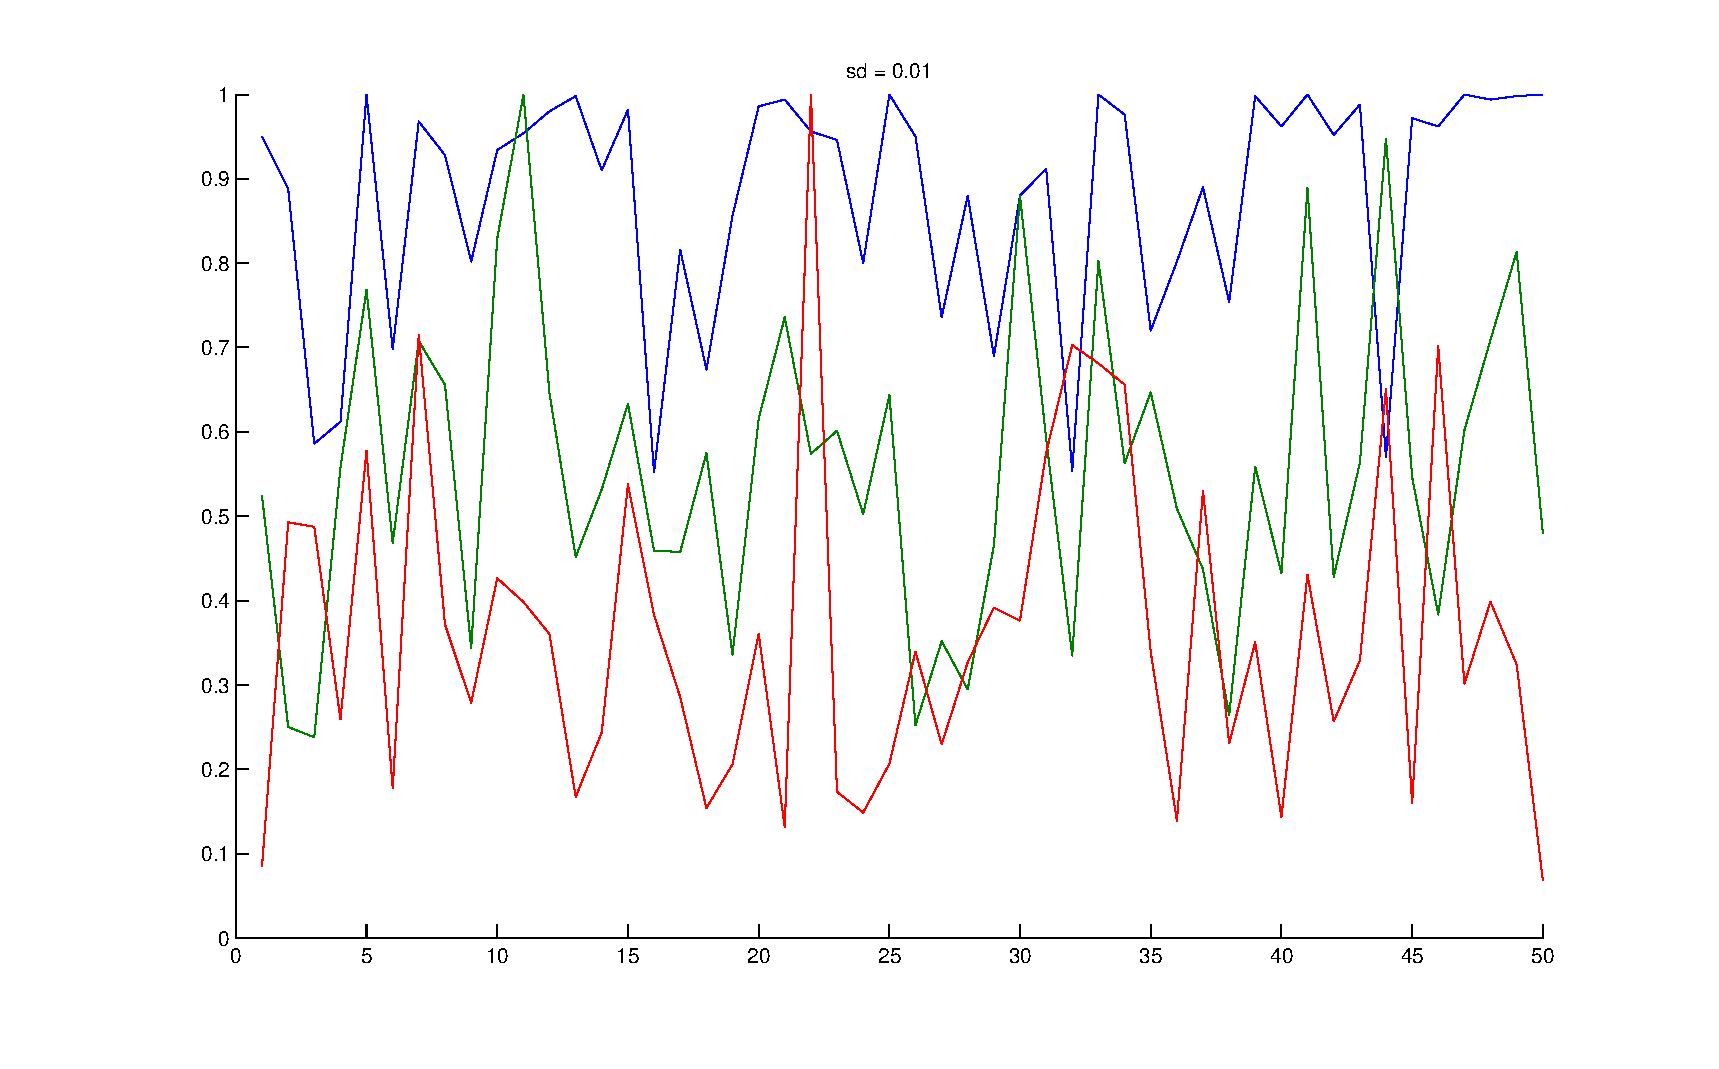
\includegraphics[width=0.45\textwidth]{results1hundredth.eps}
  \hfill
  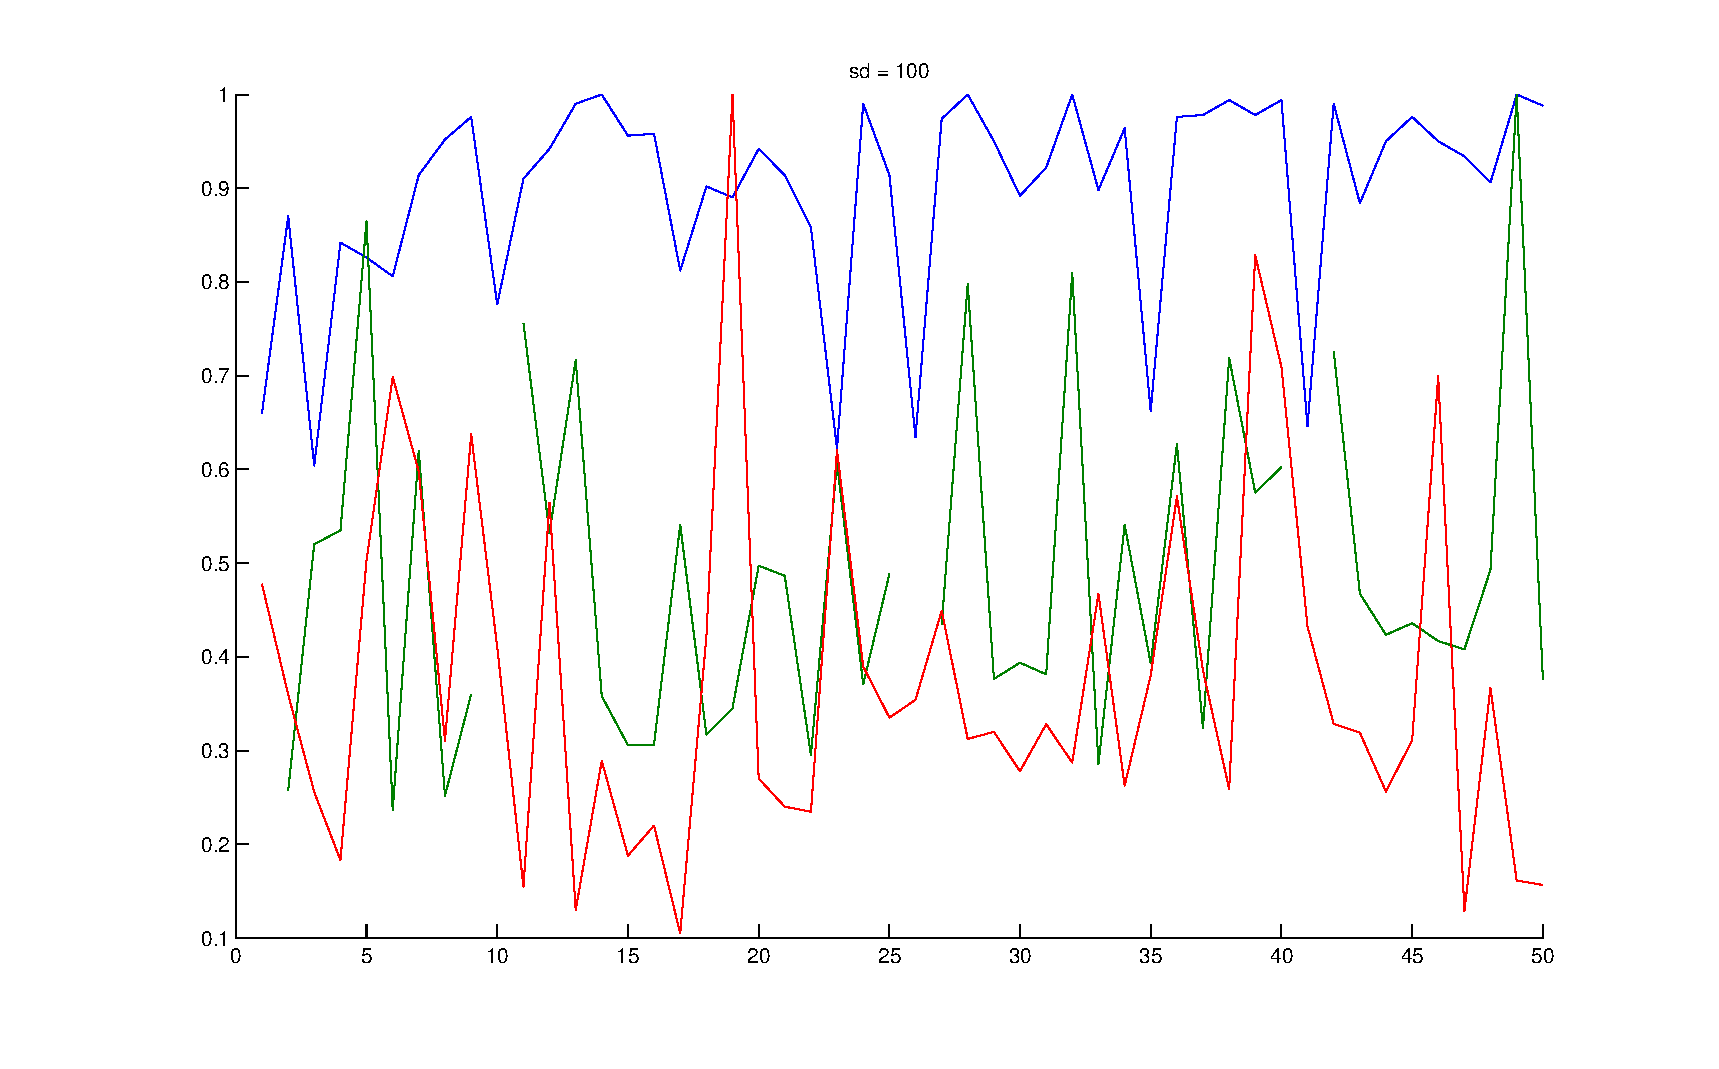
\includegraphics[width=0.45\textwidth]{results100.eps}
  \caption{The fraction correctly clustered is blue. $\mu$ is green, $\Sigma$ is red, and are both reweighted to fit within the plot (since their units are arbitary already).}
  \label{results}
\end{figure}

It's pretty easy to scale up the coded algorithm to more than two clusters, but it doesn't support more than 2 dimensions at the moment. The plots would be particularly tricky, but I don't think it would be too much more work to extend it past two dimensions. With more than two clusters, it simply requires more iterations, but it still gives pretty good results (see Figure \ref{nclusters} on the next page). The computational-intensive part is evaluating which cluster goes to which label with more than a few clusters.

\begin{figure}[h]
  \centering
  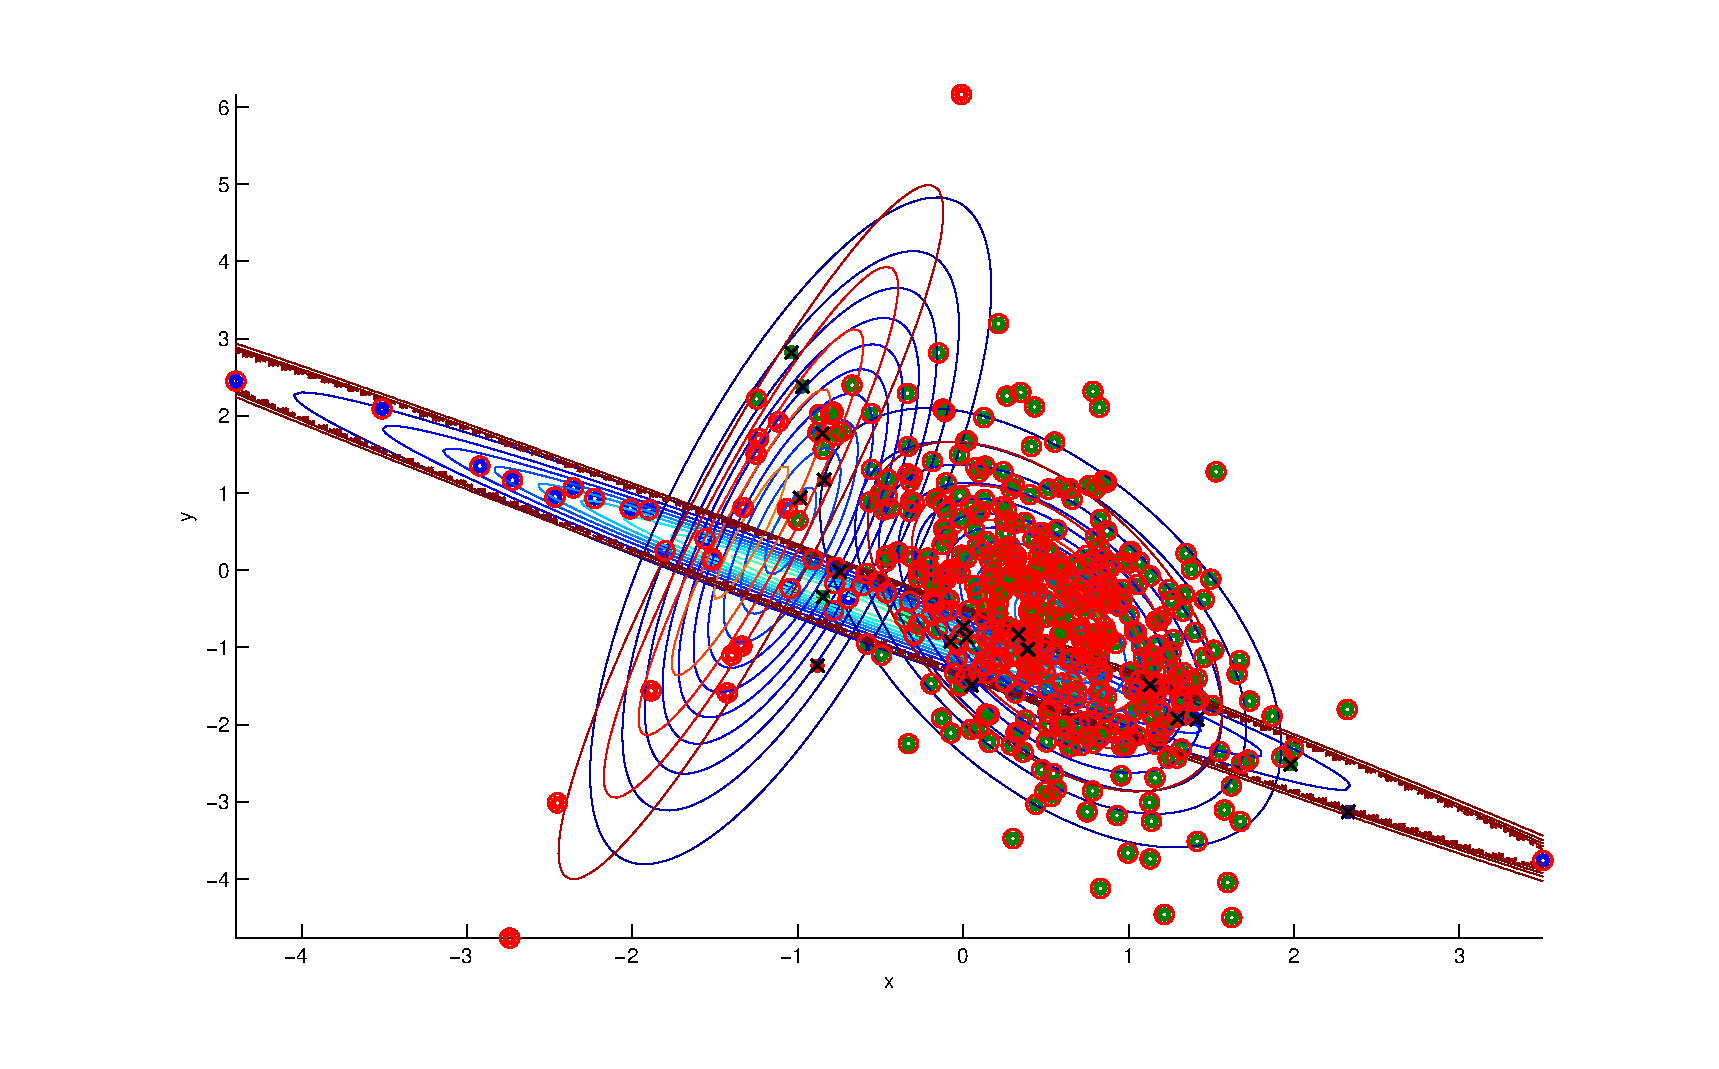
\includegraphics[width=.8\textwidth,angle=90]{nclusters3.eps}
  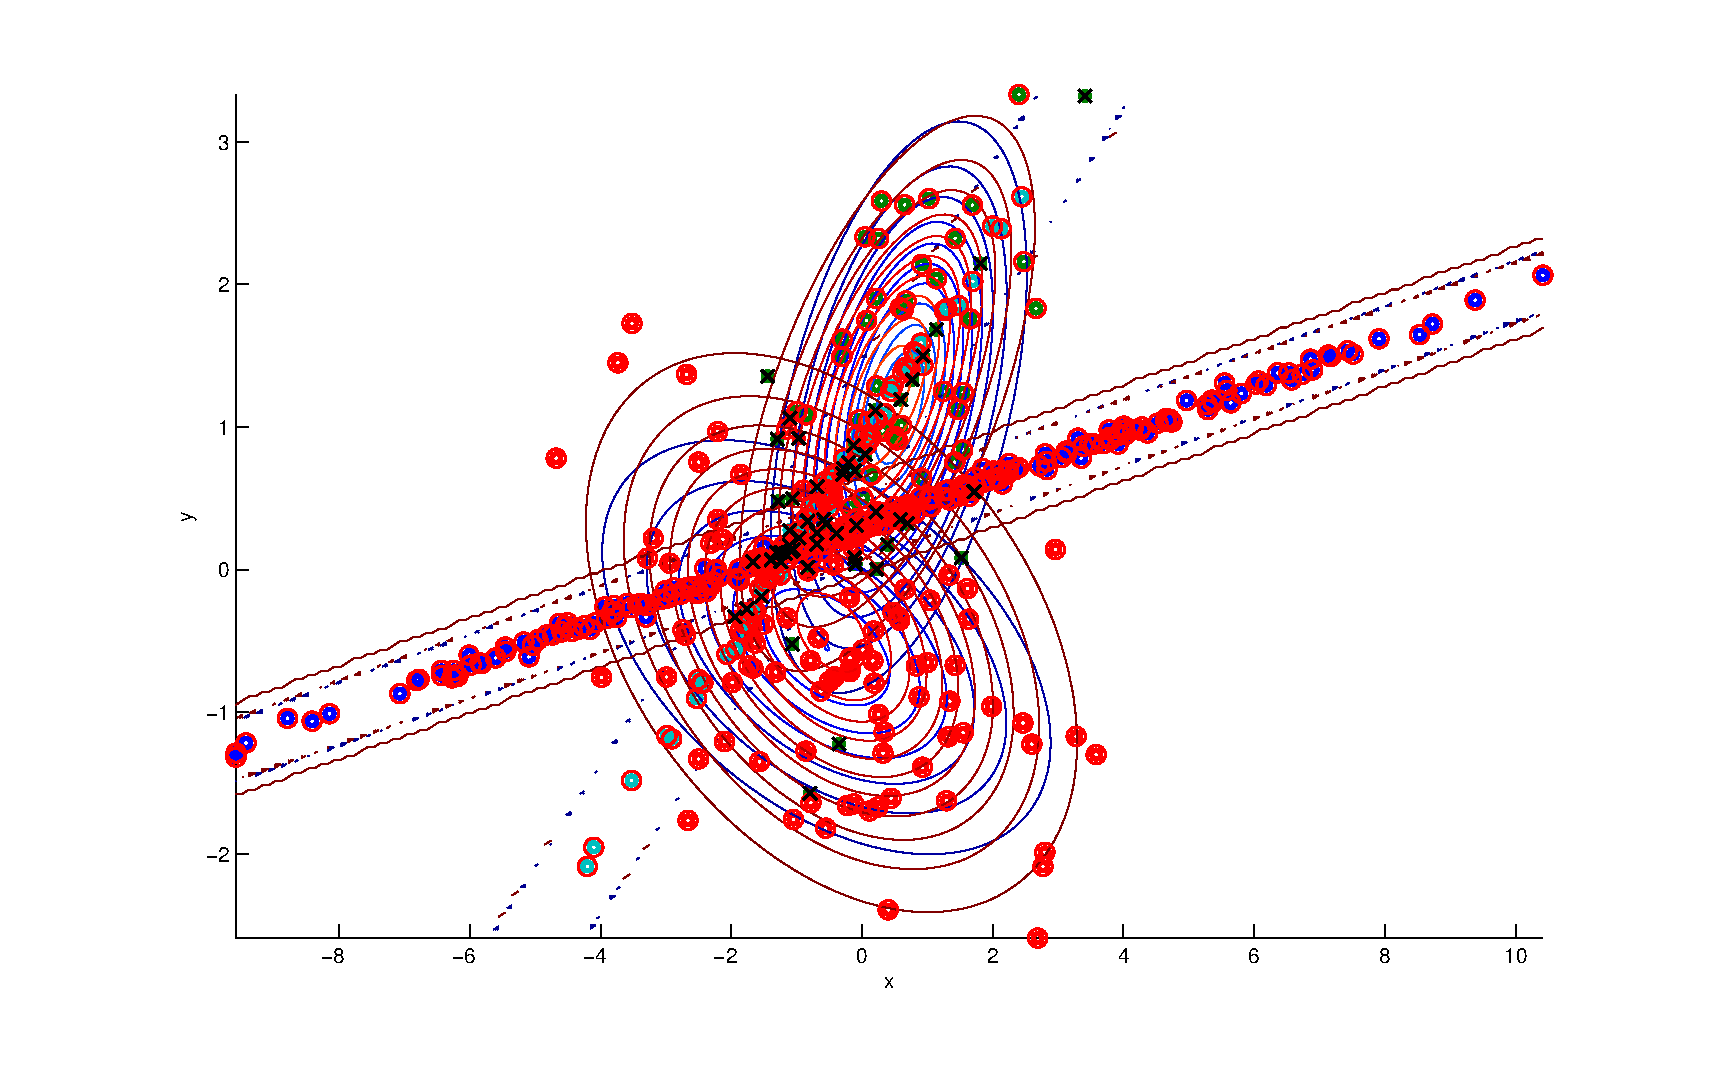
\includegraphics[width=.8\textwidth,angle=90]{nclusters4.eps}
  \vspace{-2em}
  \caption{Three, four, and seven clusters.}

  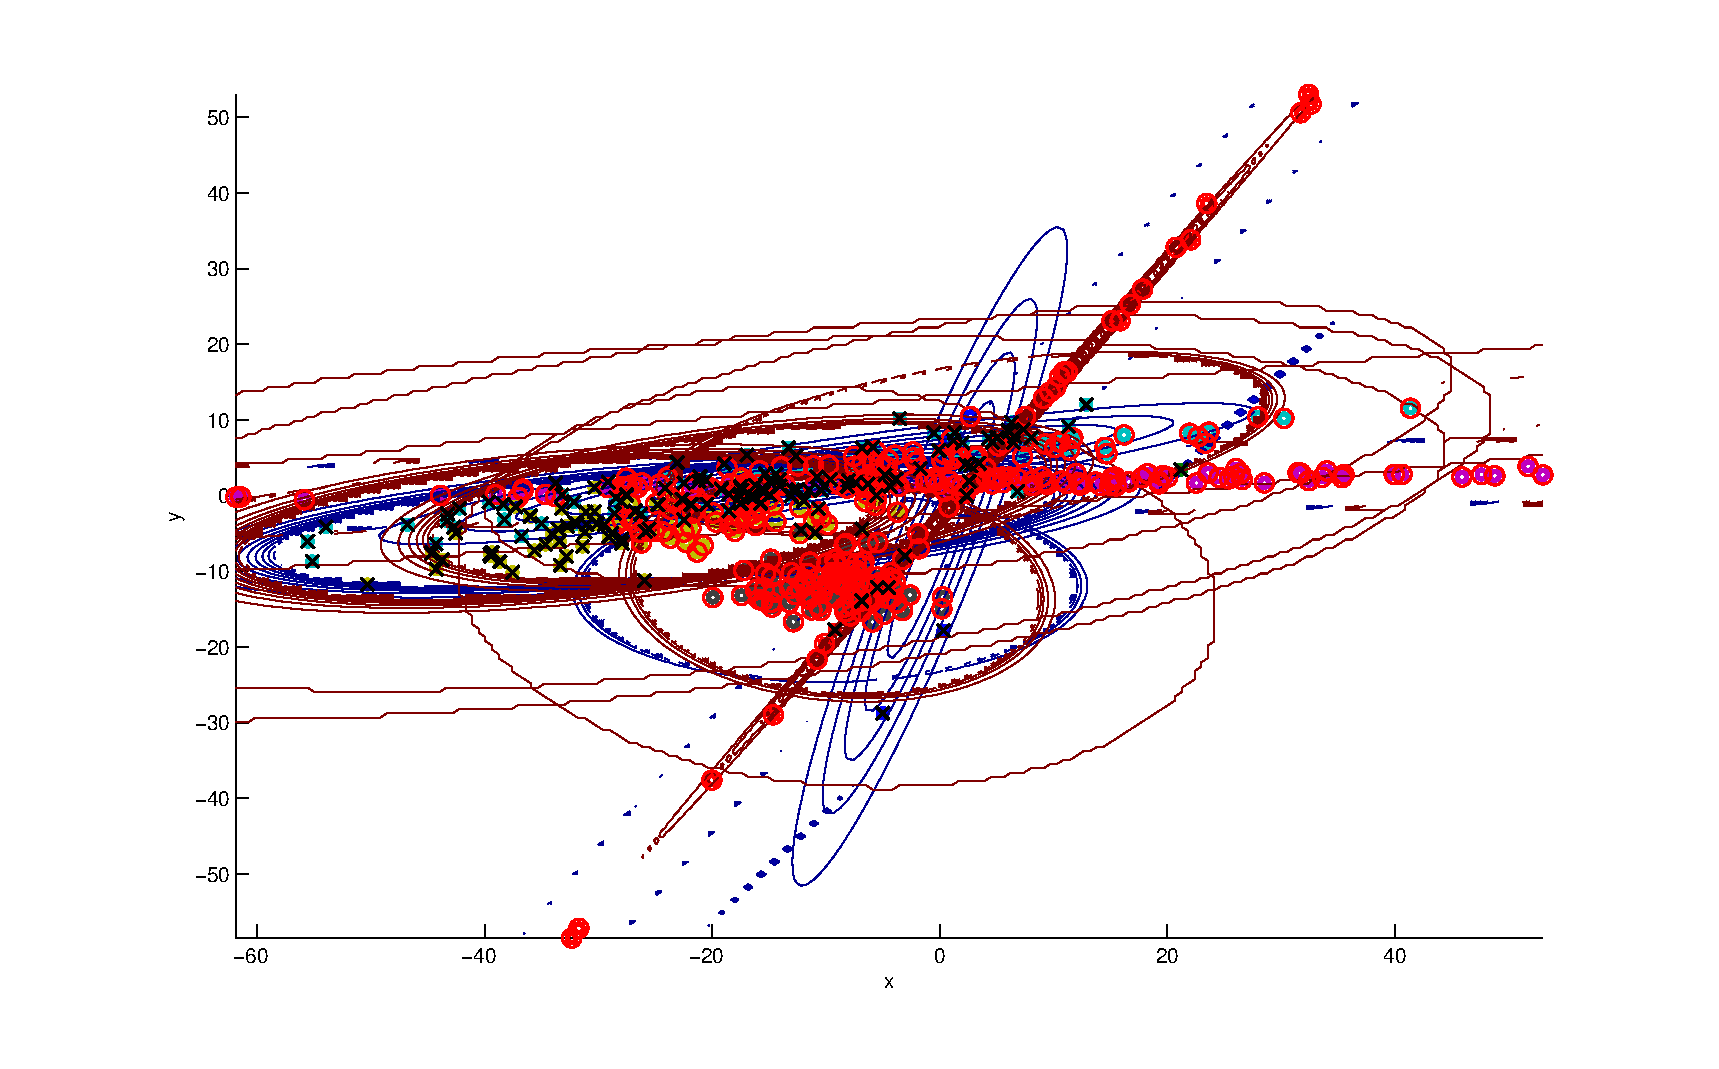
\includegraphics[width=\textwidth]{nclusters7.eps}
  \label{nclusters}
\end{figure}



% as the $\mu$ and $\Sigma$

% Describe your work in a well-written report. This should not be very long (two pages or less, unless you have a very compelling reason to wax verbose). You can use whatever method you want to generate the report (Latex, MSWord, etc), but the document you submit must be in PDF format.

% Mention implementation details (parameters used, etc.), something interesting you learned, and explain your plots. You don't need to explain the whole EM algorithhm.

\end{document}

Build a model. Randomly generate a gaussian mixture model that generates two dimensional data points. First, randomly generate two mean vectors and two covariance matricies to represent two gaussian models: 1 and 2. Also randomly generate the prior probabilities P(1) and P(2) = 1 - P(1), which control the probability of picking each of the two Gaussians.

Generate data. Generate a set of random data to use as training samples. You will likely find the MATLAB function mvnrnd helpful.

Create plots. See help plot. You must show the original data points with different colors depending on which Gaussian generated it and then show the datapoints classified according to which Gaussian your model says is most likely to have generated it. You must plot the accuracy of means and other parameters found by your algorithm compared over several trials (generate multiple sets of data) in comparison to the ground truth parameters.

Implement the Expectation Maximization algorithm You may want to use the following MATLAB functions: mvnpdf, mean, and cov. You will also need to understand different ways MATLAB provides for indexing arrays/matrices of data and for loops. Try not to use 'for...loops' when possible -- they're slow in Matlab. For more info on this, see the Matlab tutorials linked on the syllabus, or this on improving the speed of Matlab code via vectorization.

Submit. Submit your assignment before the deadline using turnin as described on the class homepage to dkit.

